\documentclass[tikz,14pt,border=10pt]{standalone}
\usepackage[T1]{fontenc}
\usepackage[latin1]{inputenc}
\usepackage[english]{babel}
\usepackage{textcomp}
\usetikzlibrary{shapes,patterns,arrows,calc,decorations.pathreplacing,positioning,graphs}
\usepackage{pgfmath}
\usepackage{tikz}
\usetikzlibrary{calc}




\begin{document}
		
	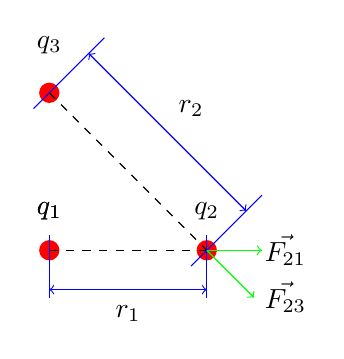
\begin{tikzpicture}[every text node part/.style={align=center},text=black, scale = 1]
	
		
		
	% connections
%	\node (q1) [] {$\mathbf{w}_{k-1}$} ;
%	\draw (0,0) coordinate (q1) --(2,1) coordinate(q2);
	\node at (0,0.5) {$q_1$};
	

	\draw[red,ultra thick, fill] (0,0) circle [radius=0.1];
	\draw[red,ultra thick,fill] (2,0) circle [radius=0.1];
	\draw[red,ultra thick,fill] (0,2) circle [radius=0.1];	
	\draw[black, dashed]  (0,0) -- (2,0);
	\draw[black, dashed]  (0,2) -- (2,0);	

	\draw[<->,blue, thin]  (0,-.5) -- (2,-0.5);
	\draw[blue] (0,-.6) -- (0,0.2);
	\draw[blue] (2,-.6) -- (2,0.2);

	\draw[<->,blue, thin]  (0.5,2.5) -- (2.5,0.5);	
	\draw[blue] (0.7,2.7) -- (-.2,1.8);
	\draw[blue] (1.8, -.2) -- (2.7,.7);
	
	\draw[green, ->] (2,0) -- (2.7,0);
	\draw[green, ->] (2,0) -- (2.6,-.6);	
	
	\node at (0,0.5) {$q_1$};
	\node at (2,0.5) {$q_2$};
	\node at (0,2.6) {$q_3$};
		
	\node at (3,0) {$\vec{F_{21}}$};	
	\node at (3,-.6) {$\vec{F_{23}}$};	
	\node at (1,-.8) {$r_1$};	
	\node at (1.8,1.8) {$r_2$};		
	\end{tikzpicture}

	
\end{document}